%
% The first command in your LaTeX source must be the \documentclass command.
\documentclass[sigplan,screen]{acmart}

%
% defining the \BibTeX command - from Oren Patashnik's original BibTeX documentation.
\def\BibTeX{{\rm B\kern-.05em{\sc i\kern-.025em b}\kern-.08emT\kern-.1667em\lower.7ex\hbox{E}\kern-.125emX}}

% Rights management information.
% This information is sent to you when you complete the rights form.
% These commands have SAMPLE values in them; it is your responsibility as an author to replace
% the commands and values with those provided to you when you complete the rights form.
%
% These commands are for a PROCEEDINGS abstract or paper.
\copyrightyear{2019}
\acmYear{2019}
\setcopyright{acmlicensed}
\acmConference[Mesa '18]{Mesa '18: SER 574}{Jan 20, 2019}{Mesa, AZ}
\acmDOI{11.2222/3333333.4444444}
\acmISBN{111-2-333-4444-1/20/19}

%
% These commands are for a JOURNAL article.
%\setcopyright{acmcopyright}
%\acmJournal{TOG}
%\acmYear{2018}\acmVolume{37}\acmNumber{4}\acmArticle{111}\acmMonth{8}
%\acmDOI{10.1145/1122445.1122456}

%
% Submission ID.
% Use this when submitting an article to a sponsored event. You'll receive a unique submission ID from the organizers
% of the event, and this ID should be used as the parameter to this command.
%\acmSubmissionID{123-A56-BU3}

%
% The majority of ACM publications use numbered citations and references. If you are preparing content for an event
% sponsored by ACM SIGGRAPH, you must use the "author year" style of citations and references. Uncommenting
% the next command will enable that style.
%\citestyle{acmauthoryear}

%
% end of the preamble, start of the body of the document source.
\begin{document}

%
% The "title" command has an optional parameter, allowing the author to define a "short title" to be used in page headers.
\title{<Title goes here>}

%
% The "author" command and its associated commands are used to define the authors and their affiliations.
% Of note is the shared affiliation of the first two authors, and the "authornote" and "authornotemark" commands
% used to denote shared contribution to the research.
\author{Paul Horton}
\email{pahorton@asu.edu}
\affiliation{%
  \institution{Arizona State University}
  \city{Mesa}
  \state{Arizona}
  \postcode{85212}
}

\author{Ruby Zhao}
\email{qrzhao@asu.edu}
\affiliation{%
  \institution{Arizona State University}
  \city{Mesa}
  \state{Arizona}
  \postcode{85212}
}

%
% The abstract is a short summary of the work to be presented in the article.
\begin{abstract}
We will write an abstract here
\end{abstract}

%
% Keywords. The author(s) should pick words that accurately describe the work being
% presented. Separate the keywords with commas.
\keywords{words, need, to, go, here}

%
% A "teaser" image appears between the author and affiliation information and the body
% of the document, and typically spans the page.
% \begin{teaserfigure}
%   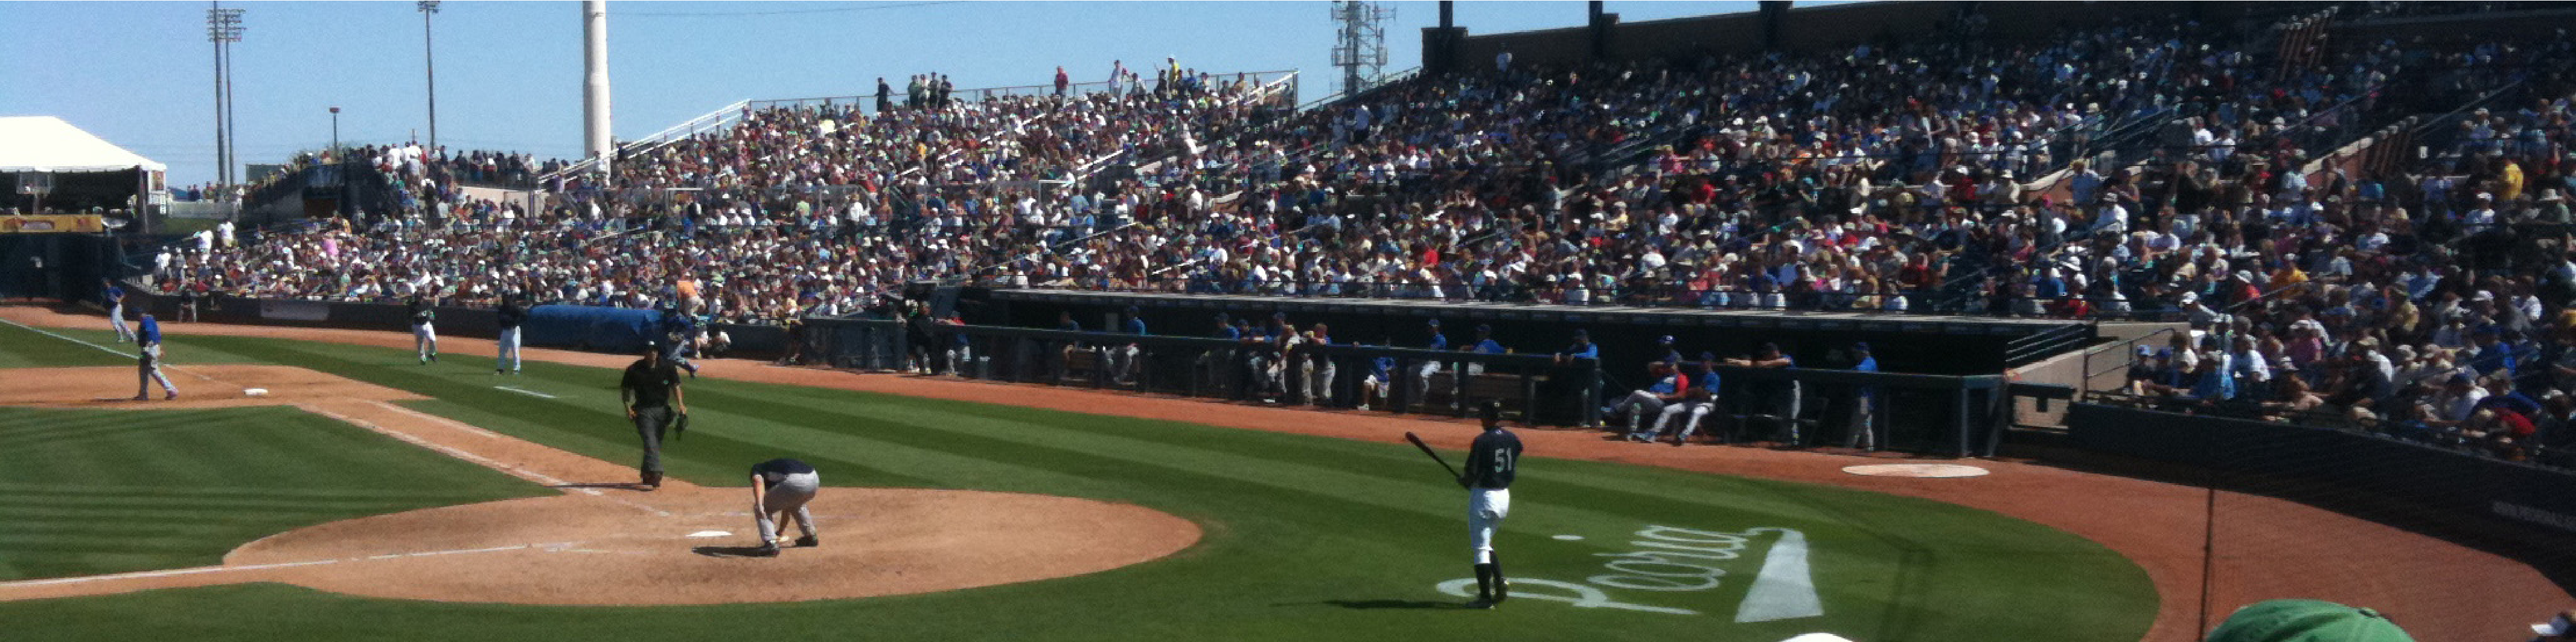
\includegraphics[width=\textwidth]{sampleteaser}
%   \caption{Seattle Mariners at Spring Training, 2010.}
%   \Description{Enjoying the baseball game from the third-base seats. Ichiro Suzuki preparing to bat.}
%   \label{fig:teaser}
% \end{teaserfigure}

%
% This command processes the author and affiliation and title information and builds
% the first part of the formatted document.
\maketitle

\section{Introduction}

\section{Template Overview}

\subsection{Template Styles}

\subsection{Template Parameters}

\section{Modifications}

\section{Typefaces}

\section{Title Information}

\section{Authors and Affiliations}

\section{Rights Information}

\section{CCS Concepts and User-Defined Keywords}

\section{Sectioning Commands}

\section{Tables}

\section{Math Equations}

%
% The next two lines define the bibliography style to be used, and the bibliography file.
\bibliographystyle{ACM-Reference-Format}
\bibliography{sample-base}


\end{document}
